\ifdefined\COMPLETE
\else
\documentclass[12pt]{article}

\usepackage{amsmath,amsthm,mathtools}
\usepackage{graphicx}
\usepackage{algorithm2e}
\usepackage{thm-restate}

\usepackage{tikz}
\usetikzlibrary{shapes, calc, arrows, through, intersections, decorations.pathreplacing, patterns}

\newtheorem{theorem}{Theorem}
\newtheorem{definition}[theorem]{Definition}
\newtheorem{thrm}[theorem]{Theorem}
\newtheorem{lem}[theorem]{Lemma}
\newtheorem{corollary}[theorem]{Corollary}

\newcommand{\mb}{\mathbf}
\newcommand{\mc}{\mathcal}
\newcommand\numberthis{\addtocounter{equation}{1}\tag{\theequation}}
\let\oldnl\nl
\newcommand{\nonl}{\renewcommand{\nl}{\let\nl\oldnl}}

\DeclareMathOperator*{\argmin}{arg\,min}
\DeclareMathOperator*{\vcdim}{VC-Dim}

\begin{document}
\fi

Modern businesses generate a tremendous amount of data which are stored in large databases. These datasets are then used to make many critical decisions. Therefore, ensuring the quality of these datasets becomes extremely important. As the data accumulates from multiple sources over time, many errors creep into the data. For example, many records end up having duplicate entries. Record de-duplication is a central task in managing large scale databases. The goal is to detect records in a database that correspond to the same real word entity. 
%Some examples of such tasks are: detecting duplicate records in a health-care dataset, duplicate customer records, duplicate publication records (in say Google Scholar) are other common examples of de-duplication tasks.

The problem of data de-duplication can be viewed as a clustering task. Here, the goal is to put records corresponding to the same physical entity in the same cluster while separating the records corresponding to different entities into different clusters. Clustering for de-duplication has many characteristics which are different from standard clustering problems. Many popular clustering algorithms like $k$-means or $k$-median receive as input the value $k$, that is the number of clusters to output. This information is unknown in de-duplication applications. In any dataset, the number of different-cluster pairs (i.e. different entity pairs) is order of magnitude greater than the number of positive or same-cluster pairs (i.e. same entity pairs). Hence, common machine learning tools of classification prediction (learning a binary classifier over the set of pairs of instances) do not automatically transfer to this domain as the dataset is heavily skewed towards the negative pairs. 

The framework of correlation clustering is very natural for modelling the problem of data de-duplication \cite{bansal2004correlation}. Here, de-duplication is viewed as an optimization problem over graphs. More formally, given a dataset $X$ and a complete graph $G$ over the set. The edges of the graph are labelled $0$ or $1$. An edge label of zero indicates that the corresponding vertices have been deemed to be in different cluster while an edge label of one indicates that the corresponding vertices should be in the same cluster. The motivation for edge labelling is the following. Often the practitioner can design a pairwise similarity function over the pairs of points. The pairs whose similarity is above a certain threshold are deemed as positive (or same-cluster) and the remaining pairs are deemed to be negative (or different-cluster). Sometimes, the similarity metric is also learned from training data. 

Given the graph, the goal of correlation clustering is to find a clustering of the dataset which correlates `as much as possible' with the given edges. In other words, find a clustering which minimizes the correlation loss w.r.t the given edges. Correlation loss is defined as the sum of the number of zero edges within a cluster plus the number of one edges across different clusters. However, solving this optimization problem is NP-Hard \cite{bansal2004correlation}. 
  
In this chapter, we offer a formal modelling of such record de-duplication tasks. Our framework is the same as correlation clustering but with the added \textit{promise} that the input graph edges $E$ is `close to' the optimal correlation clustering of the given dataset. We analyse the computational complexity of this problem and show that even under strong promise, correlation clustering is NP-Hard. Moreover, the problem remains NP-Hard (assuming the ETH hypothesis) even when we are allowed to make queries to a human expert (or an \textit{oracle}) as long as the number of queries is not too large (sub-linear in the number of points in the dataset). 

Given these negative results, we introduce the framework of restricted correlation clustering (RCC). This framework has two important differences from the standard (and promise) correlation clustering formulation. Firstly, the optimization problem is restricted over a given class $\mc F$ of clusterings. Secondly, the goal is to find a clustering which correlates as much as possible with the unknown target (or ground truth) clustering $C^*$. That is, $C^*$ is the clustering where only records corresponding to same entity are in the same cluster. We offer an algorithmic approach (which uses the help of an oracle) with success guarantees for the restricted version. The `success guarantee' depends on the complexity of the class $\mc F$ (measured by $\vcdim(\mc F)$) as well as the `closeness' of the distance (or similarity) metric $d$ to the target clustering. We complement our theoretical results by carrying out extensive experimental evaluation of our framework on a diverse class of clustering algorithms and across multiple real world datasets.

\section{Related Work}
The most relevant work is the framework of correlation clustering developed by \cite{bansal2004correlation} that we discussed in the previous section. Other variations of correlation clustering have been considered. For example \cite{demaine2006correlation}, consider a problem where the edges can be labelled by a real number instead of just $0$ or $1$. Edges with large positive weights encourage those vertices to be in the same cluster while edges with large negative weights encourage those points to be in different clusters. They showed that the problem is NP-Hard and gave a $O(\log n)$ approximation to the weighted correlation clustering problem. \cite{charikar2005clustering} made several contributions to the correlation clustering problem. For the problem of minimizing the correlation clustering loss (for unweighted complete graphs), they gave an algorithm with factor $4$ approximation. They also proved that the minimization problem is APX-Hard. 

More recently, \cite{ailon2018approximate} considered the problem of correlation clustering in the presence of an oracle. If the number of clusters $k$ is known, they proposed an algorithm which makes $O(k^{14} \log n)$ queries to the oracle and finds a $(1+\epsilon)$-approximation to the correlation clustering problem. They showed that the problem is NP-Hard to approximate with $o\big(\frac{k}{poly \log k}\big)$ queries to an oracle. In this work, we obtain similar results for the {promise correlation clustering} problem.

Supervision in clustering has been addressed before. For example, \cite{kulis2009semi,basu2004probabilistic,basu2002semi} considered {\em link/don't-link} constraints. This is a form of non-interactive clustering where the algorithm gets as input a list of pairs which should be in the same cluster and a list pairs which should be in different clusters. \cite{balcan2008clustering} developed a framework of interactive clustering where the supervision is provided in the form of {\em split/merge} queries. The algorithm gives the current clustering to the oracle. The oracle responds by telling the which clusters to merge and which clusters to split. 

In this work, we use the framework of same-cluster queries developed by \cite{ashtiani2016clustering}. At any given instant, the clustering algorithm asks the same-cluster oracle about two points in the dataset. The oracle replies by answering either `yes' or `no' depending upon whether the two points lie in the same or different clusters. 

On de-duplication side, most prevalent are approaches that are based on designing a similarity measure (or distance) over the records, such that records that are highly similar according to that measure are likely to be duplicates and records that measure as significantly dissimilar are likely to represent different entities. For example, to handle duplicate records created due typographical mistakes, many character-based similarity metrics have been considered. Examples of such metrics include the edit or levenshtein distance \cite{levenshtein1966binary}, smith-waterman distance \cite{waterman1981identification} and jaro distance metric \cite{jaro1980unimatch}. Token-based similarity metrics try to handle rearrangement of words, for example \cite{monge1996field} and \cite{cohen1998integration}. Other techniques include phonetic-based metrics and numerical metrics (to handle numeric data). A nice overview of these methods can be found in \cite{elmagarmid2007duplicate}. 
   
While the above approaches relied on designing a good similarity metric, some works try to `learn' the distance function from a labelled training dataset of pairs of records. Examples of such works include \cite{cochinwala2001efficient} and \cite{bilenko2003adaptive}. Clustering for de-duplication has been mostly addressed in application oriented works. \cite{hernandez1995merge} assumes that the duplicate records are transitive. The clustering problem now reduces to finding the connected components in a graph. \cite{hassanzadeh2009framework} carried out an extensive experimental evaluation of different graph-based clustering algorithms on a simulated dataset of strings.

\section{Preliminaries}
\label{section:problemFormulation}
Given $X$, a clustering $C$ of the set $X$ partitions it into $k$ disjoint subsets or clusters. The clustering $C$ can also be viewed as a $\{0, 1\}$-function over the domain $X^{[2]} := \{(x_1, x_2) : x_1 \neq x_2\}$. Here, $C(x_1, x_2) = 1$ iff $x_1, x_2$ belong to the same cluster according to $C$. Similarly, we also view the edges of a graph $G = (X, E)$ as a $\{0, 1\}$-function over $X^{[2]}$.

We allow a clustering algorithm to make queries to a human oracle in the following way. 
\begin{definition}[ Same-cluster oracle \cite{ashtiani2016clustering}]
Given a set $X$ and an unknown target clustering $C^*$. A same-cluster $C^*$-oracle receives a pair $(x_1, x_2) \in X^{[2]}$ as input and outputs $1$ if and only if $x_1, x_2$ belong to the same cluster according to $C^*$. 
\end{definition}
From the perspective of de-duplication, a same-cluster oracle receives two records $x_1$ and $x_2$. The oracle returns $1$ if $x_1$ and $x_2$ correspond to the same real-world entity. Otherwise, the oracle responds $0$.

\begin{definition}[Correlation loss\cite{bansal2004correlation}]
\label{defn:correlationLoss}
Given graph $G = (X, E)$ where $X$ is the set of vertices (the given dataset to be clustered) and $E$ is the set of edges. The correlation loss of a clustering $C$ w.r.t the edges $E$ is defined as \begin{align*}
  &corrL_{E}(C) = corrN_{E}(C) + corrP_{E}(C), \text{ where}\\
  corrN_{E}(C) &= |\{(x, y): C(x, y) = 1 \text{ and } E(x, y) = 0\}|,\\ 
  corrP_{E}(C) &= |\{(x, y): C(x, y) = 0 \text{ and } E(x, y) = 1\}| \numberthis\label{eqn:correlationLoss}
\end{align*}
A weighted version of the loss function places weights of $w_1$ and $w_2$ on the two terms and is defined as 
\begin{align}
  &corrL_{E}^{w}(C) = w_1 \thinspace corrN_{E}(C) + w_2 \thinspace corrP_{E}(C)\label{eqn:weightedCorrelationLoss}
\end{align}
\end{definition}

The goal of correlation clustering is to find a clustering which minimizes the (weighted) correlation loss. We also consider the normalized version of this loss function w.r.t a target clustering $C^*$ (rather than the edges $E$).

\begin{definition}[Normalized correlation loss]
\label{defn:normalizedCorrelationLoss}
Given domain $X$, a target clustering $C^*$ and a parameter $\mu$. The loss of a clustering $C$ w.r.t the target $C^*$ is defined as
\begin{align*}
  L_{C^*}(C) &= \enspace  \mu \enspace L_{P^+}(C) \enspace+\enspace (1-\mu) \enspace L_{P^-}(C), \text{ where} \\
  &L_{P^+}(C) = \underset{(x, y) \sim P^+}{\mb P} \big[ C(x, y) = 0 ],\\
  & L_{P^-}(C) = \underset{(x, y) \sim P^-}{\mb P} \big[ C(x, y) = 1] \numberthis\label{eqn:RCCV2}
\end{align*}
where $P^+$ is the uniform distribution over $X^{[2]}_+ = \{(x, y) : C^*(x, y) = 1\}$ and $P^-$ is the uniform distribution over $X^{[2]}_- = \{(x, y): C^*(x, y) = 0\}$. 
\end{definition}
The normalized correlation loss measures two quantities for the clustering $C$. The first is the fraction of the true positive pairs that $C$ gets wrong (or loss over the positive pairs). The second is the fraction of true negative pairs that $C$ gets wrong (or the loss over the negative pairs). It then obtains a weighted sum of the two losses. 
  
Lets observe the relation between Defns. \ref{defn:correlationLoss} and \ref{defn:normalizedCorrelationLoss}. Define $\gamma_0 := \mb P[C^*(x, y) = 1]$, that is the probability of true positive (or same-cluster pairs) in the dataset. Using the notation of Defn. \ref{defn:correlationLoss}, we see that $corrP_{C^*}(C) = \gamma_0|X^{[2]}| L_{P^+}(C)$ and $corrN_{C^*}(C) = (1-\gamma_0)|X^{[2]}| L_{P^-}(C)$. Normalising by $|X^{[2]}|$ and choosing $\mu = \frac{w_2 \gamma_0}{w_1 (1-\gamma_0) + w_2 \gamma_0}$ gives us the normalized version of the loss function.

\begin{definition}
\label{defn:informativeMetric}
Given a metric space $(X, d)$, a target clustering $C^*$ and a parameter $\lambda$. We say that the metric $d$ is $(\alpha, \beta)$-informative w.r.t $C^*$ and $\lambda$ if
\begin{align}
	&\underset{(x, y) \sim U^2}{\mb P}\enspace \big[d(x, y) > \lambda \enspace|\enspace C^*(x, y) = 1\big] \enspace \le \enspace \alpha \label{eqn:alphaInformative}\\
	&\underset{(x, y) \sim U^2}{\mb P}\enspace \big[C^*(x, y) = 1 \enspace|\enspace d(x, y) \le \lambda \big] \enspace \ge \enspace \beta \label{eqn:betaInformative}
\end{align}
Here $U^2$ is the uniform distribution over $X^{[2]}$. 
\end{definition} 
In deduplication applications, often the distance function is such that pairs with distance within a certain threshold are likely to be in the same cluster. The definition of an informative metric formalizes this intuition. It says that most of the true positive pairs have a distance of atmost $\lambda$ between them. Also, amongst all pairs with distance $\le \lambda$, atleast a $\beta$ fraction of them belong to the same cluster. 

\begin{definition}[$\gamma$-skewed] 
\label{defn:gammaskewed} 
Given $X$ and a target clustering $C^*$. We say that $X$ is $\gamma$-skewed w.r.t $C^*$ if 
\begin{align*}
	&\underset{(x, y) \sim U^2}{\mb P}\enspace \big[\enspace C^*(x, y) = 1 \big] \enspace \le \enspace \gamma
\end{align*}
\end{definition}
In de-duplication applications, most of the pairs are negative (or belong to different clusters). The above definition states this property formally. In the next section, we introduce our framework of \textit{promise correlation clustering} and discuss the computational complexity of the problem both in the absence and presence of an oracle.   

\section{Promise Correlation Clustering}
\label{section:PCC}

\begin{definition}[Promise correlation clustering (PCC)]
\label{defn:promiseCorrClustering}
Given a clustering instance $G = (X, E)$. Let $C^*$ be such that
\begin{align}
  &C^* = \argmin_{C \in \mc F} \enspace corrL_{E}(C) \label{eqn:promiseCorrLoss}
\end{align}
where $\mc F$ is the set of all possible clusterings $C$ such that $m(C) \le p$. Given that $E$ is $(\alpha, \beta)$-informative w.r.t $C^*$. Find the clustering $C^*$. 
\end{definition}
When the edges $E$ correspond to a clustering $C$ then $\beta = 1$ and $\alpha = 0$. We show in the subsequent sections that even for this `restricted' class of clusterings (when the size of the maximum cluster is atmost a constant $M$) and given the prior knowledge, PCC is still NP-Hard. Furthermore, PCC is NP-Hard even when we are allowed to make $o(|X|)$ queries to a $C^*$-oracle. 

\subsection{PCC is NP-Hard}
\label{section:PCCNPHard}
\begin{figure*}[!ht]
	\centering
	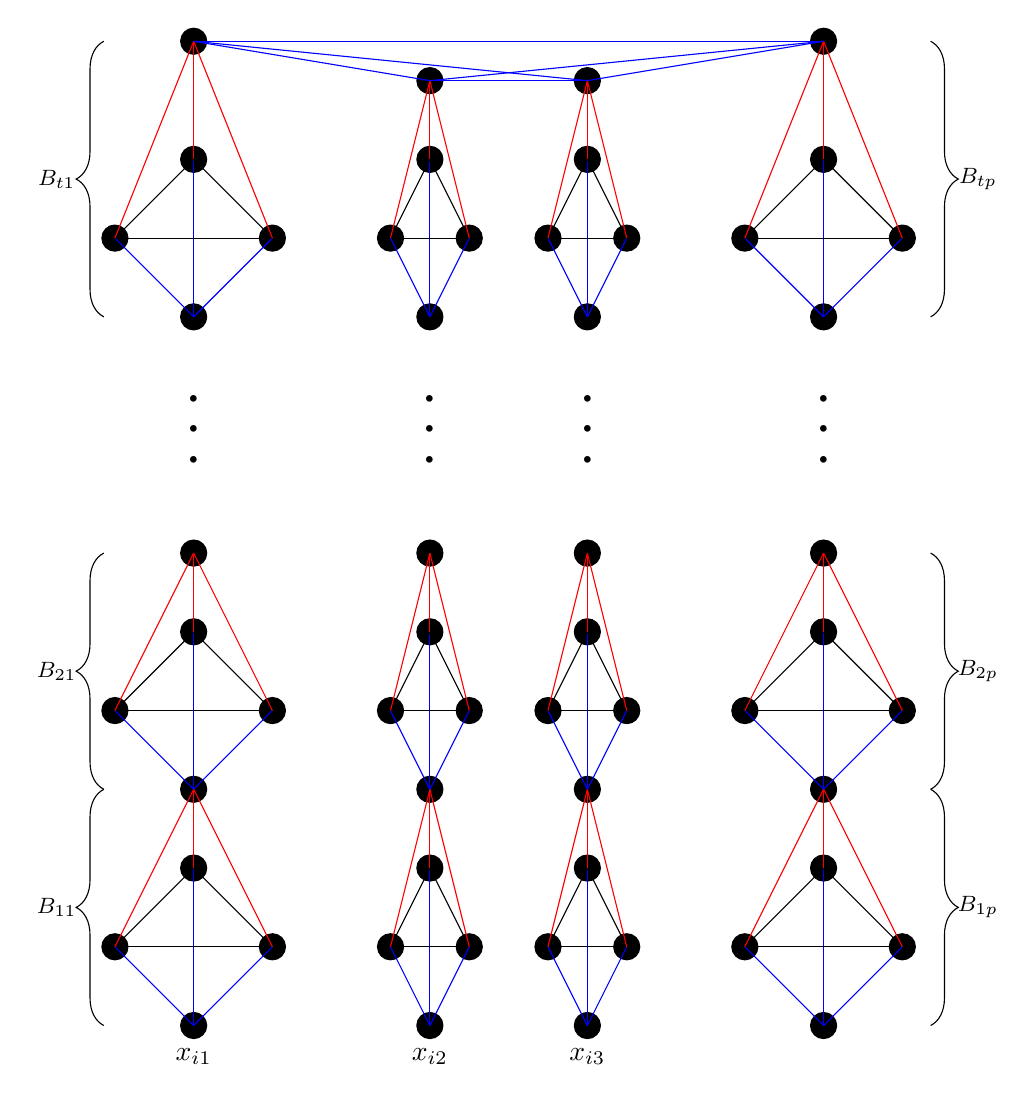
\begin{tikzpicture}
	  \node[circle,draw,minimum size=1mm,,fill=black,label=below:$x_{i1}$] at (0, 0){};
	  \node[circle,draw,fill=black] at (0, 2){};
	  \node[circle,draw,fill=black] at (-1, 1){};
	  \node[circle,draw,fill=black] at (1, 1){};
	  \node[circle,draw,fill=black] at (0, 3){};

	  \node[circle,draw,fill=black] at (0, 5){};
	  \node[circle,draw,fill=black] at (-1, 4){};
	  \node[circle,draw,fill=black] at (1, 4){};
	  \node[circle,draw,fill=black] at (0, 6){};
			
	  \node[circle,draw,fill=black] at (0, 9){};
	  \node[circle,draw,fill=black] at (0, 11){};
	  \node[circle,draw,fill=black] at (-1, 10){};
	  \node[circle,draw,fill=black] at (1, 10){};
	  \node[circle,draw,fill=black] at (0, 12.5){};
	
	  \draw[blue] (0, 0) -- (0, 2);
	  \draw[blue] (0, 0) -- (-1, 1);
	  \draw[blue] (0, 0) -- (1, 1);
	  \draw (1, 1) -- (-1, 1);
	  \draw (1, 1) -- (0, 2);
	  \draw (-1, 1) -- (0, 2);
	  \draw[red] (1, 1) -- (0, 3);
	  \draw[red] (-1, 1) -- (0, 3);
	  \draw[red] (0, 3) -- (0, 2);
		
	  \draw[blue] (0, 3) -- (0, 5);
	  \draw[blue] (0, 3) -- (-1, 4);
	  \draw[blue] (0, 3) -- (1, 4);
	  \draw (1, 4) -- (-1, 4);
	  \draw (1, 4) -- (0, 5);
	  \draw (-1, 4) -- (0, 5);
	  \draw[red] (1, 4) -- (0, 6);
	  \draw[red] (-1, 4) -- (0, 6);
	  \draw[red] (0, 6) -- (0, 5);
	
	  \draw[blue] (0, 9) -- (0, 11);
	  \draw[blue] (0, 9) -- (-1, 10);
	  \draw[blue] (0, 9) -- (1, 10);
	  \draw (1, 10) -- (-1, 10);
	  \draw (1, 10) -- (0, 11);
	  \draw (-1, 10) -- (0, 11);
	  \draw[red] (1, 10) -- (0, 12.5);
	  \draw[red] (-1, 10) -- (0, 12.5);
	  \draw[red] (0, 12.5) -- (0, 11);
	  	
	  \node[circle,draw,minimum size=1mm,,fill=black,label=below:$x_{i2}$] at (3, 0){};
	  \node[circle,draw,fill=black] at (3, 2){};
	  \node[circle,draw,fill=black] at (2.5, 1){};
	  \node[circle,draw,fill=black] at (3.5, 1){};
	  \node[circle,draw,fill=black] at (3, 3){};
	
	  \node[circle,draw,fill=black] at (3, 5){};
	  \node[circle,draw,fill=black] at (2.5, 4){};
	  \node[circle,draw,fill=black] at (3.5, 4){};
	  \node[circle,draw,fill=black] at (3, 6){};
		
	  \node[circle,draw,fill=black] at (3, 9){};
	  \node[circle,draw,fill=black] at (3, 11){};
	  \node[circle,draw,fill=black] at (2.5, 10){};
	  \node[circle,draw,fill=black] at (3.5, 10){};
	  \node[circle,draw,fill=black] at (3, 12){};
	  		
	  \draw[blue] (3, 0) -- (3, 2);
	  \draw[blue] (3, 0) -- (2.5, 1);
	  \draw[blue] (3, 0) -- (3.5, 1);
	  \draw (3.5, 1) -- (2.5, 1);
	  \draw (3.5, 1) -- (3, 2);
	  \draw (2.5, 1) -- (3, 2);
	  \draw[red] (2.5, 1) -- (3, 3);
	  \draw[red] (3.5, 1) -- (3, 3);
	  \draw[red] (3, 3) -- (3, 2);
	  
	  \draw[blue] (3, 3) -- (3, 5);
	  \draw[blue] (3, 3) -- (2.5, 4);
	  \draw[blue] (3, 3) -- (3.5, 4);
	  \draw (3.5, 4) -- (2.5, 4);
	  \draw (3.5, 4) -- (3, 5);
	  \draw (2.5, 4) -- (3, 5);
	  \draw[red] (3.5, 4) -- (3, 6);
	  \draw[red] (2.5, 4) -- (3, 6);
	  \draw[red] (3, 6) -- (3, 5);
	  
	  \draw[blue] (3, 9) -- (3, 11);
	  \draw[blue] (3, 9) -- (2.5, 10);
	  \draw[blue] (3, 9) -- (3.5, 10);
	  \draw (3.5, 10) -- (2.5, 10);
	  \draw (3.5, 10) -- (3, 11);
	  \draw (2.5, 10) -- (3, 11);
	  \draw[red] (3.5, 10) -- (3, 12);
	  \draw[red] (2.5, 10) -- (3, 12);
	  \draw[red] (3, 12) -- (3, 11);
	  
	  \node[circle,draw,minimum size=1mm,,fill=black,label=below:$x_{i3}$] at (5, 0){};
	  \node[circle,draw,fill=black] at (5, 2){};
	  \node[circle,draw,fill=black] at (4.5, 1){};
	  \node[circle,draw,fill=black] at (5.5, 1){};
	  \node[circle,draw,fill=black] at (5, 3){};
	
	  \node[circle,draw,fill=black] at (5, 5){};
	  \node[circle,draw,fill=black] at (4.5, 4){};
	  \node[circle,draw,fill=black] at (5.5, 4){};
	  \node[circle,draw,fill=black] at (5, 6){};
		
	  \node[circle,draw,fill=black] at (5, 9){};
	  \node[circle,draw,fill=black] at (5, 11){};
	  \node[circle,draw,fill=black] at (4.5, 10){};
	  \node[circle,draw,fill=black] at (5.5, 10){};
	  \node[circle,draw,fill=black] at (5, 12){};
	  		
	  \draw[blue] (5, 0) -- (5, 2);
	  \draw[blue] (5, 0) -- (4.5, 1);
	  \draw[blue] (5, 0) -- (5.5, 1);
	  \draw (5.5, 1) -- (4.5, 1);
	  \draw (5.5, 1) -- (5, 2);
	  \draw (4.5, 1) -- (5, 2);
	  \draw[red] (5.5, 1) -- (5, 3);
	  \draw[red] (4.5, 1) -- (5, 3);
	  \draw[red] (5, 3) -- (5, 2);
	  
	  \draw[blue] (5, 3) -- (5, 5);
	  \draw[blue] (5, 3) -- (4.5, 4);
	  \draw[blue] (5, 3) -- (5.5, 4);
	  \draw (5.5, 4) -- (4.5, 4);
	  \draw (5.5, 4) -- (5, 5);
	  \draw (4.5, 4) -- (5, 5);
	  \draw[red] (5.5, 4) -- (5, 6);
	  \draw[red] (4.5, 4) -- (5, 6);
	  \draw[red] (5, 6) -- (5, 5);
	  
	  \draw[blue] (5, 9) -- (5, 11);
	  \draw[blue] (5, 9) -- (4.5, 10);
	  \draw[blue] (5, 9) -- (5.5, 10);
	  \draw (5.5, 10) -- (4.5, 10);
	  \draw (5.5, 10) -- (5, 11);
	  \draw (4.5, 10) -- (5, 11);
	  \draw[red] (5.5, 10) -- (5, 12);
	  \draw[red] (4.5, 10) -- (5, 12);
	  \draw[red] (5, 12) -- (5, 11);
	  
	  \node[circle,draw,minimum size=1mm,fill=black] at (8, 0){};
	  \node[circle,draw,fill=black] at (8, 2){};
	  \node[circle,draw,fill=black] at (7, 1){};
	  \node[circle,draw,fill=black] at (9, 1){};
	  \node[circle,draw,fill=black] at (8, 3){};

	  \node[circle,draw,fill=black] at (8, 5){};
	  \node[circle,draw,fill=black] at (7, 4){};
	  \node[circle,draw,fill=black] at (9, 4){};
	  \node[circle,draw,fill=black] at (8, 6){};
			
	  \node[circle,draw,fill=black] at (8, 9){};
	  \node[circle,draw,fill=black] at (8, 11){};
	  \node[circle,draw,fill=black] at (7, 10){};
	  \node[circle,draw,fill=black] at (9, 10){};
	  \node[circle,draw,fill=black] at (8, 12.5){};
	
	  \draw[blue] (8, 0) -- (8, 2);
	  \draw[blue] (8, 0) -- (7, 1);
	  \draw[blue] (8, 0) -- (9, 1);
	  \draw (9, 1) -- (7, 1);
	  \draw (9, 1) -- (8, 2);
	  \draw (7, 1) -- (8, 2);
	  \draw[red] (9, 1) -- (8, 3);
	  \draw[red] (7, 1) -- (8, 3);
	  \draw[red] (8, 3) -- (8, 2);
		
	  \draw[blue] (8, 3) -- (8, 5);
	  \draw[blue] (8, 3) -- (7, 4);
	  \draw[blue] (8, 3) -- (9, 4);
	  \draw (9, 4) -- (7, 4);
	  \draw (9, 4) -- (8, 5);
	  \draw (7, 4) -- (8, 5);
	  \draw[red] (9, 4) -- (8, 6);
	  \draw[red] (7, 4) -- (8, 6);
	  \draw[red] (8, 6) -- (8, 5);
	
	  \draw[blue] (8, 9) -- (8, 11);
	  \draw[blue] (8, 9) -- (7, 10);
	  \draw[blue] (8, 9) -- (9, 10);
	  \draw (9, 10) -- (7, 10);
	  \draw (9, 10) -- (8, 11);
	  \draw (7, 10) -- (8, 11);
	  \draw[red] (9, 10) -- (8, 12.5);
	  \draw[red] (7, 10) -- (8, 12.5);
	  \draw[red] (8, 12.5) -- (8, 11);
	
	  \draw[blue] (0, 12.5) -- (8, 12.5);
	  \draw[blue] (0, 12.5) -- (5, 12);
	  \draw[blue] (0, 12.5) -- (3, 12);
	  \draw[blue] (3, 12) -- (5, 12);
	  \draw[blue] (3, 12) -- (8, 12.5);
	  \draw[blue] (5, 12) -- (8, 12.5);
	  
	  \path (0, 9) -- (0, 6) node [black, font=\Huge, midway, sloped] {$\dots$};
	  \path (3, 9) -- (3, 6) node [black, font=\Huge, midway, sloped] {$\dots$};
	  \path (5, 9) -- (5, 6) node [black, font=\Huge, midway, sloped] {$\dots$};
	  \path (8, 9) -- (8, 6) node [black, font=\Huge, midway, sloped] {$\dots$};
	  
	  \draw [decorate,decoration={brace,amplitude=10pt},xshift=-4pt,yshift=0pt]
(-1,0) -- (-1,3) node [black,midway,xshift=-0.6cm] 
{\footnotesize $B_{11}$};
	  \draw [decorate,decoration={brace,amplitude=10pt},xshift=-4pt,yshift=0pt]
(-1,3) -- (-1,6) node [black,midway,xshift=-0.6cm] 
{\footnotesize $B_{21}$};
	  \draw [decorate,decoration={brace,amplitude=10pt},xshift=-4pt,yshift=0pt]
(-1,9) -- (-1,12.5) node [black,midway,xshift=-0.6cm] 
{\footnotesize $B_{t1}$};
	  \draw [decorate,decoration={brace,amplitude=10pt,mirror},xshift=-4pt,yshift=0pt]
(9.5,0) -- (9.5,3) node [black,midway,xshift=0.6cm] 
{\footnotesize $B_{1p}$};
	  \draw [decorate,decoration={brace,amplitude=10pt,mirror},xshift=-4pt,yshift=0pt]
(9.5,3) -- (9.5,6) node [black,midway,xshift=0.6cm] 
{\footnotesize $B_{2p}$};
	  \draw [decorate,decoration={brace,amplitude=10pt,mirror},xshift=-4pt,yshift=0pt]
(9.5,9) -- (9.5,12.5) node [black,midway,xshift=0.6cm] 
{\footnotesize $B_{tp}$};
	\end{tikzpicture}
\caption{Part of graph $G$ constructed for the subset $S_i =  \{x_{i1}, x_{i2}, x_{i3}\}$. The graph is constructed by local replacement for $p = 4$. The vertices labeled $x_{ij}$ correspond to the elements in the universe $U$. If $S_i$ is included in the exact cover then the edges colored black and the edges colored blue represent the corresponding clustering of this part of the graph $G$. If $S_i$ is not included in the exact cover then the edges colored red and the edges colored black represent the clustering of this part of the graph.}
\label{fig:X3CNPHard}
\end{figure*}

\begin{theorem}
Finding the optimal solution to the Promise Correlation Clustering problem is NP-Hard for all $p \ge 3$ and for $\alpha = 0$ and $\beta = \frac{1}{2}$.  
\end{theorem}

\noindent To prove the result, we will use a reduction from exact cover by $3$-sets problem which is known to be NP-Hard.

(X3C) Given a universe of elements $U = \{x_1, \ldots, x_{3q}\}$ and a collections of subsets $S = \{S_1, \ldots, S_m\}$. Each $S_i \subset U$ and contains exactly three elements. Does there exist $S' \subseteq S$ such that each element of $U$ occurs exactly once in $S'$?

This decision problem is known to be NP-Hard \cite{garey2002computers}. We will now reduce an instance of X3C to the promise correlation clustering problem using local replacement described in Fig. \ref{fig:X3CNPHard}. The details of the construction are as follows. For every element $x \in U$, we add a corresponding vertex $x \in V$. For every three set $S_i = \{x_{i1}, x_{i2}, x_{i3}\}$, we construct $B_{ij}$ for $i \le t$ and $j \le p$. Here, $t$ is a constant which will be specified later. Each $B_{ij}$ is a clique of size $p$. The `connection' between the different blocks are specified in Fig. \ref{fig:X3CNPHard}. Let $A$ be an algorithm which solves the promise problem described in Eqn. \ref{eqn:promiseCorrLoss}. Then, we can use this algorithm to decide exact cover by three sets as follows.

If $A$ outputs a clustering $C$ such that all the clusters have size exactly $p$ and $E_C$ makes no negative errors w.r.t $E$ (that is $\alpha(E_C) = 0$) then output YES. Otherwise, output NO. Next, we will prove that this procedure decides X3C. 

Let there exists an exact cover for the X3C instance. Let $C$ be the clustering corresponding to the exact cover. That is, the edges colored blue and black correspond to this clustering and the corresponding vertices are in the same cluster (Fig. \ref{fig:X3CNPHard}). Note that this clustering makes no negative errors. Furthermore, each point is in a cluster of size exactly $p$. Thus, the positive error corresponding to any vertex is the degree of that vertex minus $p-1$. Since, the size of a cluster is atmost $p$, this is the minimum possible positive error for any vertex. Hence, any other clustering strictly makes more positive errors than $C$. 

It is easy to see from the construction that if $A$ finds a clustering which has no negative errors and all the clusters have size $p$, then this corresponds to exact cover of the X3C instance and hence we output YES. If this does not happen then there does not exist any exact cover for $(U, S)$. This is because if there was an exact cover then the corresponding clustering would satisfy our condition. Thus, $A$ decides X3C. Since, X3C is NP-Hard, no polynomial time algorithm $A$ exists unless $P = NP$.

In the construction, for each clause, we have $p^2 t + (p - 3)$ vertices and a vertex for each of the variables. Therefore, $|V| = m (p^2 t + (p-3)) + 3q$ and $|E| = pt({p \choose 2}+p-1) + {p \choose 2}$.  Consider a clustering $C$ which places all the $x_i$'s  and $r_i$'s in singleton clusters and places rest of the points in clusters of size $p$. For $t \ge 2$,
\begin{align*}
  \beta &= \frac{pt{p \choose 2}}{pt({p \choose 2}+p-1) + {p \choose 2}} = \frac{1}{1 + \frac{2}{p} + \frac{1}{pt}} > \frac{1}{2} \text{ and }\alpha = 0
\end{align*} 

\subsection{Hardness of PCC in the presence of an oracle}
\label{section:PCCNPHardOracle}
In the previous sections, we have shown that the PCC problem is NP-Hard without queries. It is trivial to see that if $\alpha = 0$ then making $\beta |X|$ queries to the same-cluster oracle allows us to solve (in polynomial time) the Promise Correlation Clustering problem for all $p$. In this section, we prove that the linear dependence on $n = |X|$ is tight if we assume that the exponential time hypothesis (ETH) is correct. 

ETH is an assumption about computational hardness of the 3SAT problem. The non-uniform version of ETH (which we will use in this section) posits that there does not exist an algorithm that can solve 3-SAT in $2^{o(n)}$ time. We prove that if the exponential time hypothesis (ETH) holds then any algorithm that runs in polynomial time makes atleast $\Omega(n)$ same-cluster queries. The main idea is to reduce 3SAT to our problem. We do this by the following sequence of reductions, 3SAT to 3DM to X3C to PCC. These reductions show that (under ETH) the running time of PCC is $2^{o(n)}$. Using a `simulation trick' we then prove that any query-based algorithm for PCC needs to make atleast $\Omega(n)$ queries.

\begin{theorem}
Given that the Exponential Time Hypothesis (ETH) holds then any algorithm for the Promise Correlation Clustering problem  that runs in polynomial time makes $\Omega(|X|)$ same-cluster queries for all $p \ge 3$ and for $\alpha = 0$ and $\beta = \frac{1}{2}$. 
\end{theorem}

\noindent We will now prove the above theorem. We state the definition of the different problems used in the reduction.
\begin{definition}[3-SAT].\\
Input: A boolean formulae $\phi$ in 3CNF with $n$ literals and $m$ clauses. Each clause has exactly three literals. \\
Output: YES if $\phi$ is satisfiable, NO otherwise. 
\end{definition}

\begin{definition}[3DM].\\
Input: Sets $W, X$ and $Y$ and a set of matches $M \subseteq W \times X \times Y$ of size $m$.  \\
Output: YES if there exists $M' \subseteq M$ such that each element of $W, X, Y$ appears exactly once in $M'$. NO otherwise. 
\end{definition}

\noindent To prove that (X3C) is NP-Hard, the standard We will reduce 3-SAT to 3-dimensional matching problem. 3DM is already known to be NP-Hard. However, the standard reduction of 3-SAT to 3DM constructs a set with $|M| \in \Theta(m^2 n^2)$. Hence, using the standard reduction, the exponential time hypothesis would imply there does not exist an algorithm for 3DM which runs in $\Omega(m^\frac{1}{4})$. Our reduction is based on the standard reduction. However, we make some clever optimizations especially in the way we encode the clauses. This helps us improve the lower bound to $\Omega(m)$.

\begin{figure}[!ht]
	\centering
	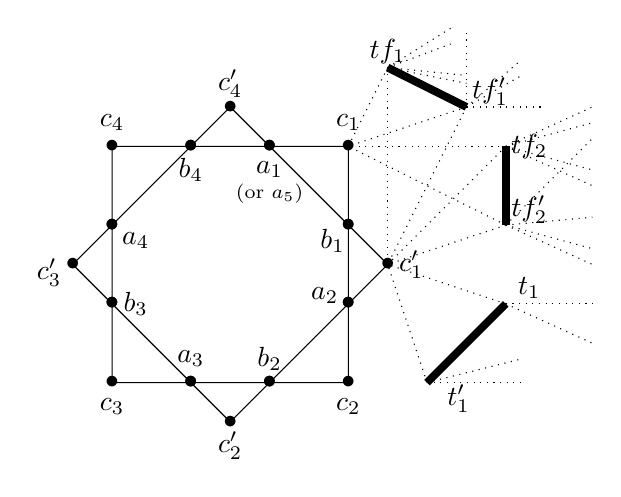
\begin{tikzpicture}
	  \draw (0,0) node {$\bullet$} -- (1,0) node{$\bullet$} -- (0.5,0.5) node{$\bullet$} -- cycle;
	  \draw (1,0) node{$\bullet$} -- (2,0) node{$\bullet$}
  -- (2,-1) node{$\bullet$} -- cycle;
	  \draw (2,-1) node{$\bullet$} -- (2,-2) node{$\bullet$} -- (2.5,-1.5) node{$\bullet$} -- cycle;
	  \draw (2,-2) node{$\bullet$} -- (1,-3) node{$\bullet$} -- (2,-3) node{$\bullet$} -- cycle;
	  \draw (0,-3) node{$\bullet$} -- (1,-3) node{$\bullet$} -- (0.5,-3.5) node{$\bullet$} -- cycle;
	  \draw (0,-3) node{$\bullet$} -- (-1,-2) node{$\bullet$} -- (-1,-3) node{$\bullet$} -- cycle;
	  \draw (-1,-2) node{$\bullet$} -- (-1,-1) node{$\bullet$} -- (-1.5,-1.5) node{$\bullet$} -- cycle;
	  \draw (0,0) node{$\bullet$} -- (-1,-1) node{$\bullet$} -- (-1,0) node{$\bullet$} -- cycle;
	
	 \node  at (0.0,-0.3) {$b_4$};
	 \node  at (1.0,-0.3) {$a_1$};
	 \node  at (1.0,-0.6) {\scriptsize{(or $a_5$)}};
	 \node  at (2.0,0.3) {$c_1$};
	 \node  at (1.8,-1.2) {$b_1$};
	 \node  at (1.7,-1.9) {$a_2$};
	 \node  at (2.8,-1.5) {$c_1'$};
	 \node  at (2.0,-3.3) {$c_2$};
	 \node  at (1.0,-2.7) {$b_2$};
	 \node  at (0.0,-2.7) {$a_3$};
	 \node  at (0.5,-3.8) {$c_2'$};
	 \node  at (-1.0,-3.3) {$c_3$};
	 \node  at (-0.7,-2.0) {$b_3$};
	 \node  at (-0.7,-1.2) {$a_4$};
	 \node  at (-1.8,-1.6) {$c_3'$};
	 \node  at (-1.0,0.3) {$c_4$};
	 \node  at (0.5,0.8) {$c_4'$};
	 
	 \node  at (2.5,1.2) {$tf_1$};
	 \node  at (3.8,0.7) {$tf_1'$};
	 \node  at (4.3,0.0) {$tf_2$};
	 \node  at (4.3,-0.8) {$tf_2'$};
	 \node  at (4.3,-1.8) {$t_1$};
	 \node  at (3.4,-3.2) {$t_1'$};

	 \draw [line width=1mm] (4,0) -- (4,-1);
	 %\node  at (4.3,-0.5) {$\gamma_i$};
	 \draw [line width=1mm] (2.5,1) -- (3.5,0.5);
	 %\node  at (3.2,0.9) {$\beta_i$};
	 \draw [line width=1mm] (4,-2) -- (3,-3);
  	 %\node  at (3.8,-2.6) {$\alpha_i$};
	 
  	\draw[dotted](4, 0) -- (2, 0);
  	\draw[dotted](4, -1) -- (2, 0);
  	\draw[dotted](4, 0) -- (2.5, -1.5);
  	\draw[dotted](4, -1) -- (2.5, -1.5);
  	\draw[dotted](4, 0) -- (5.1, 0.5);
  	\draw[dotted](4, 0) -- (5.1, 0.3);
  	\draw[dotted](4, 0) -- (5.1, -0.5);
  	\draw[dotted](4, 0) -- (5.1, -0.3);
  	\draw[dotted](4, -1) -- (5.1, 0.1);
  	\draw[dotted](4, -1) -- (5.1, -0.9);
  	\draw[dotted](4, -1) -- (5.1, -1.5);
  	\draw[dotted](4, -1) -- (5.1, -1.3);

  	\draw[dotted](2.5, 1) -- (2, 0);
  	\draw[dotted](3.5, 0.5) -- (2, 0);
  	\draw[dotted](2.5, 1) -- (2.5, -1.5);
  	\draw[dotted](3.5, 0.5) -- (2.5, -1.5);
  	\draw[dotted](2.5, 1) -- (3.3, 1.5);
  	\draw[dotted](2.5, 1) -- (3.3, 1.3);
  	\draw[dotted](2.5, 1) -- (3.5, 0.9);
  	\draw[dotted](2.5, 1) -- (3.5, 0.8);
  	\draw[dotted](3.5, 0.5) -- (4.2, 1.1);
  	\draw[dotted](3.5, 0.5) -- (4.2, 0.9);
  	\draw[dotted](3.5, 0.5) -- (3.5, 1.5);
  	\draw[dotted](3.5, 0.5) -- (4.5, 0.5);

  	\draw[dotted](4, -2) -- (2.5, -1.5);
  	\draw[dotted](3, -3) -- (2.5, -1.5);
  	\draw[dotted](4, -2) -- (5.1, -2);
  	\draw[dotted](4, -2) -- (5.1, -2.5);
  	\draw[dotted](3, -3) -- (4.2, -3);
  	\draw[dotted](3, -3) -- (4.2, -2.7);
  	\end{tikzpicture}
  	\caption{Part of graph $G$ constructed for the literal $x_1$. The figure is an illustration for when $x_1$ is part of four different clauses. The triangles (or hyper-edge) $(a_i, b_i, c_i)$ capture the case when $x_1$ is true and the other triangle $(b_i, c_i', a_{i+1})$ captures the case when $x_1$ is false. Assuming that a clause $C_j = \{x_1, x_2, x_3\}$, the hyper-edges containing $tf_i, tf_i'$ and $t_1, t_1'$ capture different settings. The hyper-edges containing $t_1, t_1'$ ensure that atleast one of the literals in the clause is true. The other two ensure that two variables can take either true or false values.}
\label{fig:3DMQueries}
\end{figure}

Our gadget is described in Fig. \ref{fig:3DMQueries}. For each literal $x_i$, let $m_i$ be the number of clauses in which the the literal is present. We construct a ``truth-setting" component containing $2m_i$ hyper-edges (or triangles). We add the following hyper-edges to $M$.
\begin{align*}
  &\{(a_k[i], b_k[i], c_k[i]): 1 \le k \le m_i\} \cup \{(a_{k+1}[i], b_k[i], c_k'[i]): 1 \le k \le m_i\}
\end{align*}
Note that one of $(a_k, b_k, c_k)$ or $(a_{k+1}, b_k, c_k')$ have to be selected in a matching $M'$. If the former is selected that corresponds to the variable $x_i$ being assigned true, the latter corresponds to false. This part is the same as the standard construction. 

For every clause $C_j = \{x_1, x_2, x_3\}$ we add three types of hyper-edges.  The first type ensures that atleast one of the literals is true. 
$$\{(c_k[i], t_1[j], t_1'[j]): x_i' \in C_j\} \cup \{(c_k'[i], t_1[j], t_1'[j]): x_i \in C_j\}$$ 
The other two types of hyper-edges (conected to the $tf_i$'s) say that two of the literals can be either true or false. Hence, we connect them to both $c_k$ and $c_k'$
\begin{align*}
  &\{(c_k[i], tf_1[j], tf_1'[j]): x_i' \text{ or }x_i\in C_j\} \cup \{(c_k[i], tf_2[j], tf_2'[j]): x_i \text{ or }x_i' \in C_j\}\\
  &\cup \{(c_k'[i], tf_1[j], tf_1'[j]): x_i' \text{ or }x_i\in C_j\} \cup \{(c_k'[i], tf_2[j], tf_2'[j]): x_i \text{ or }x_i' \in C_j\}
\end{align*}
Note that in the construction $k$ refers to the index of the clause $C_j$ in the truth-setting component corresponding to the literal $x_i$. Using the above construction, we get that
\begin{align*}
  & W = \{c_k[i], c_k'[i]\}\\
  & X = \{a_k[i]\} \cup \{t_1[j], tf_1[j], tf_2[j]\}\\
  & Y = \{b_k[i]\} \cup \{t_1'[j], tf_1'[j], tf_2'[j]\}
\end{align*} 
Hence, we see that $|W| = 2\sum_i m_i = 6m$. Now, $|X| = |Y| = \sum_i m_i + 3m = 6m$. And, we have that $|M| = 2\sum_i m_i + 15m = 21m$. Thus, we see that this construction is linear in the number of clauses. 

Now, if the 3-SAT formula $\phi$ is satisfiable then there exists a matching $M'$ for the 3DM problem. If a variable $x_i = T$ in the assignment then add $(c_k[i], a_k[i], b_k[i])$ to $M'$ else add $(c_k'[i], a_{k+1}[i], b_k[i])$. For every clause $C_j$, let $x_i$ (or $x_i'$) be the variable which is set to true in that clause. Add $(c_k'[i], t_1[j], t_1'[j])$  (or $(c_k[i], t_1[j], t_1'[j])$) to $M'$. For the remaining two clauses, add the hyper-edges containing $tf_1[j]$ and $tf_2[j]$ depending upon their assignments. Clearly, $M'$ is a matching. 

Now, the proof for the other direction is similar. If there exists a matching, then one of $(a_k, b_k, c_k)$ or $(a_{k+1}, b_k, c_k')$ have to be selected in a matching $M'$. This defines a truth assignment of the variables. Now, the construction of the clause hyper-edges ensures that every clause is satisfiable.

\begin{theorem}
If the exponential time hypothesis holds then there does not exist an algorithm which decides the three dimensional matching problem 3DM and runs in time $2^{o(m)}$.
\end{theorem}

\begin{corollary}
\label{cor:X3CLowerBound}
If the exponential time hypothesis holds then there does not exist an algorithm which decides exact cover by 3-sets problem (X3C) and runs in time $2^{o(m)}$.
\end{corollary}

Hence, from the discussion in this section, we know that X3C is not only NP-Hard but the running time is lower bounded by $\Omega(2^m)$. Now, using the same reduction of X3C to PCC as before, gives the same lower bound on the running time of PCC. Using this, we can now lower bound the number of queries required by PCC.

For the sake of contradiction, let us assume that there exists an algorithm which solves PCC in polynomial time by making $o(n)$ same-cluster queries ($n$ is the number of vertices). Then by simulating all possible answers for the oracle, we get a non-query algorithm which solves PCC in $2^{o(n)}$. However, combining Cor. \ref{cor:X3CLowerBound} with the reduction of X3C to PCC, we get that any algorithm that solves PCC takes $\Omega(2^n)$. Hence, no such query algorithm exists. 

\ifdefined\COMPLETE
\else
\end{document}
\fi